\documentclass[12pt,a4paper]{report}


\usepackage{amsmath,amsthm,amssymb}

\usepackage[utf8]{inputenc}
\usepackage[russian]{babel}
\usepackage[T2A]{fontenc}

\usepackage{mathtext}
\usepackage{graphicx}

\usepackage{cmap}


\DeclareMathSizes{12}{14}{10}{8}

\usepackage[left=30mm, right=15mm, top=20mm, bottom=20mm]{geometry}
\usepackage{indentfirst}
\usepackage{setspace}
\usepackage{multirow,makecell,array}
\usepackage{cite} 
\usepackage{enumerate}
\hyphenpenalty=10000 

%\usepackage{float}
\usepackage{floatrow}
\usepackage{calc}

\makeatletter
\bibliographystyle{utf8gost705u}
\usepackage{titlesec}
\usepackage[usenames]{color}
\usepackage{colortbl}
\setcounter{secnumdepth}{5} 
\usepackage{tocloft} 

\renewcommand{\tiny}{\fontsize{7}{8.4pt}\selectfont}
\renewcommand{\scriptsize}{\fontsize{9}{11pt}\selectfont}
\renewcommand{\footnotesize}{\fontsize{11}{13.6pt}\selectfont}
\renewcommand{\small}{\fontsize{12}{14.5pt}\selectfont}
\renewcommand{\normalsize}{\fontsize{14}{18pt}\selectfont}
\renewcommand{\large}{\fontsize{17}{20pt}\selectfont}
\renewcommand{\Large}{\fontsize{20}{25pt}\selectfont}

\usepackage{hyperref}
\providecommand{\phantomsection}{}


\newcommand{\ket}[1]{\left|#1\right\rangle}
\newcommand{\bra}[1]{\left\langle #1\right|}

\newcommand{\NL}[2]{#1_{\mbox{\tiny #2}}}

\newcommand{\VSD}{\NL{V}{SD}}
\newcommand{\VG}{\NL{V}{G}}
\newcommand{\kBT}{k_{\mbox{\tiny B}}T}
\newcommand{\sgn}{\mbox{sgn}}

\newcommand{\Cis}[1]{C^{\mbox{\tiny о}}_{#1}}
\newcommand{\hCis}{\hat{C}^{\mbox{\tiny о}}}
\newcommand{\Cel}[1]{C^{\mbox{\tiny э}}_{#1}}
\newcommand{\hCel}{\hat{C}^{\mbox{\tiny э}}}
\newcommand{\Cisel}[1]{C^{\mbox{\tiny о-э}}_{#1}}
\newcommand{\hCisel}{\hat{C}^{\mbox{\tiny о-э}}}

\newcommand{\qis}{q^{\mbox{\tiny о}}}
\newcommand{\qel}{q^{\mbox{\tiny э}}}
\newcommand{\nis}{n^{\mbox{\tiny о}}}
\newcommand{\nel}{n^{\mbox{\tiny э}}}
\newcommand{\phiis}{\phi^{\mbox{\tiny о}}}
\newcommand{\phiel}{\phi^{\mbox{\tiny э}}}


\usepackage{ulem}
\usepackage{xcolor}
\definecolor{emerald}{rgb}{0.31, 0.78, 0.47}
\newcommand{\rdout}[1]{{\color{red}\sout{#1}}}
\newcommand{\gradd}[1]{{\color{emerald}#1}}
\newcommand{\oradd}[1]{{\color{orange}#1}}
\newcommand{\bradd}[1]{{\color{blue}#1}}
\newcommand{\subrg}[2]{{\color{red}\sout{#1}}{\color{OliveGreen}#2}}

\DeclareFloatSeparators{mysep}{\hspace{1cm}}%какая-то штука для картинок в ряд, вроде расстояние между плавающими объектами
\DeclareFloatSeparators{mysep2}{\hspace{2cm}}

\begin{document}
\section*{Приветствие}
Добрый день! Отчёт по тестовому заданию для вас подготовил Назаров Степан. Вот мой телефон: +79152827651 и почта: nazarov.ss17@physics.msu.ru
% настройка отступов
\setlength{\parindent}{1.25cm} 
% убираем висячие строки  и подобное безобразие
\sloppy   
% Запрещаем разрыв страницы после первой строки абзаца
\clubpenalty=10000		
% Запрещаем разрыв страницы перед последней строкой абзаца
\widowpenalty=10000		

% Полуторный интервал
\onehalfspacing
%титульник
\thispagestyle{empty}


\setcounter{page}{1}
\tableofcontents

\chapter*{Задание 1}
\addcontentsline{toc}{chapter}{Задание 1}

Первое задание, по сравнению со вторым, кажется вполне решаемым и скорее техническим. Говоря по сути, нужно просто подгрузить данные в датафрейм с помощью pandas в правильной кодировке, сгруппировать их по необходимым критериям и проверить статистические гипотезы. Весь процесс отражён в ноутбуке severstal 1.ipynb. Здесь же предлагаю кратко обсудить эту проверку гипотез.
\section*{Первая гипотеза}
\addcontentsline{toc}{section}{Первая гипотеза}
Необходимо обосновать, что более 3 бракованных листов на партию выходит значимо чаще для стали марки А, чем для стали марки B.

Рассчитаем количество записей в таблице для стали марок A и B. Получим $n_a = 139$ и $n_b = 98$ соответственно. Теперь посчитаем количество записей, когда в партии для каждой из марок более трёх бракованных листов. Получим $x_a = 53$ и $x_b = 44$ соответственно. Заметим, что:
\begin{equation}
\frac{x_a}{n_a} \approx 0.38 < 0.45 \approx \frac{x_b}{n_b}
\end{equation}

И тут возникает некоторая проблема, т.к. банальные значения статистических частот противоречат тому, что от нас требуется доказать. Может быть, в задании имелось в виду, что в среднем число бракованных листов для стали марки A больше чем для стали марки B, при рассмотрении случаев с числом бракованных листов в партии больше 3. Это тоже можно проверить с помощью модификации T-теста из пакета scipy. Для этого из выборок с помощью функции describe из pandas вытащим средние, стандартные отклонения и количество наблюдений. Но p-value в итоге всё равно получается больше 0.05, а значит нулевую гипотезу о равенстве средних, мы отклонить не можем.

Резюмируя всё выше сказанное, имеем полное право утверждать, что предлагаемая статистическая гипотеза неверна.
\section*{Вторая гипотеза}
\addcontentsline{toc}{section}{Вторая гипотеза}
При скоростях прокатки более 4 м/с свыше 3 бракованных листов стали на партию выходит значимо чаще, чем при меньших скоростях прокатки. Забегая вперёд: с этой гипотезой всё в порядке.

Как и прежде, начинаем с группировки данных. Составим выборку только из тех случаев, когда на партию больше трёх бракованных листов. Марка стали — любая.

Теперь разобьём эту выборку на две подвыборки: в первой скорости проката больше четырёх, во второй скорость проката меньше, либо равна 4. 

Количество наблюдений в первой подвыборке $n_> = 74$, а во второй $n_{\leq} = 23$. И пускай тут уже всё ясно и очевидно, но просто для строгости проведём статистический тест $\chi^2$. Нулевая гипотеза: частотности при разбиении по категориальному признаку не отличаются от ожидаемых. Альтернативная: отличаются. Иными словами, если предлагаемая нам для доказательства гипотеза не верна, и от скорости проката ничего бы  не зависело, мы бы получили $n_> \approx n_{\leq} \approx 48.5 = \frac{74 + 23}{2}$ — ожидаемая частотность. Рассчитываем p-value и получаем число в районе $10^{-12}$, что позволяет нам отклонить нулевую гипотезу. Таким образом, получаем, что категориальное разбиение данных по "threshold'у" скорости статистически значимо.

Внимательный читатель наверняка заметит, что мы доказали лишь только значимость скорости, а не то, что вероятность отнесения к первой группе, больше чем ко второй. В принципе для этого тоже есть статистический тест, но поизучав документацию к scipy, я его там не нашёл. Пример расчёта необходимой статистики показан на рис.\ref{fig:test}, где $u_{кр}$ — квантиль требуемого уровня значимости(по умолчанию 0.05) для стандартного нормального распределения, $\Phi_0$ — функция ошибок 
\begin{figure}[h]
	\center{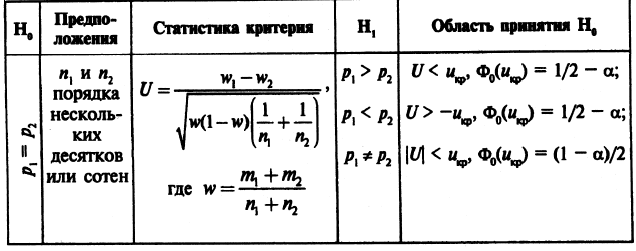
\includegraphics[scale=0.8]{test.png}}
	\caption{Статистика}
	\label{fig:test}
\end{figure}

Всё же, прибегать к этой статистике на данном этапе — скорее уже экзотика. Ведь с помощью критерия $\chi^2$ мы показали, что разбиение по категориальному признаку неравномерно и оно статистически значимо, а вероятнее первая группа, или вторая можно увидеть уже, что называется, методом пристального взгляда.

\chapter*{Задание 2}
\addcontentsline{toc}{chapter}{Задание 2}
А вот это уже настоящая брутальная задача, где проверяется стойкость характера.
\section*{Модель}
\addcontentsline{toc}{section}{Модель}
Для того, чтобы понять, в какую сторону двигаться, вероятно, необходимо некоторое погружение в тему термической обработки металлов. Где-то на подкорке мозга вашего покорного слуги завалялась информация о том, что конечные свойства металла определяются историей температурного режима. Закалка, отпуск, нормализация, цементация. Не всегда все эти процессы применяют к одному и тому же куску стали, но, например, закалка, а потом отпуск имеют место быть.

Собственно, о чём вообще речь? Мы знаем, что лист проводит в печи ровно один час, проходя последовательно между несколькими камерами. Причём температурный режим, между камерами может и должен отличаться существенно.

Каждую минуту мы снимаем с 17 датчиков показания, что определяют на выходе число — качество стали.

Заглянем в данные и посмотрим, сколько у нас уникальных значений качества стали:

\begin{figure}[h]
	\center{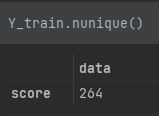
\includegraphics[scale=0.8]{N.jpg}}
	\caption{Количество уникальных качеств стали в датасете}
	\label{fig:test}
\end{figure}

Лирическое отступление: после этого стало немного грустно, ибо мы понимаем, что будем решать задачу регрессии, а не классификации ввиду следущих обстоятельств:
\begin{description}

\item[\itshape (a)] Максимальное значение score(качество стали) в датасете $score_{max} = 505$, минимальное — $score_{min} = 221$. $score_{max} - score_{min} = 284$, что не сходится с количеством уникальных скоров $score_{unique} = 264$. А значит имеем дело с пропущенными значениями, которые модель классификации не сможет определить.
\item[\itshape (b)] Погуглив в интернетах, как ведёт себя алгоритм классического ML Random forest, например, на таком количестве классов и фичей(об этом ниже), понимаем, что ведёт он себя скверно.(\url{https://stats.stackexchange.com/questions/56758/maximum-number-of-classes-for-randomforest-multiclass-estimation})
\end{description}
В сухом остатке мы имеем в качестве "иксов" $17 * 60 = 1020$ чисел, снятых с датчиков, с помощью которых нам нужно предсказать один "игрек" — марку стали. В качестве baseline'а будем использовать все данные за предыдущий час. Да может, не все из этих 1020 чисел одинаковы важны, но об этом пока думать не будем. В качестве модели будем писать нейронную сеть на Pytorch.

Важное замечание: в данных у нас есть время каждого из измерений. Оглядываясь на мой опыт работы в лаборатории, времена технологических процессов приходилось подстраивать в завсисимости от времени года, ибо зимой скажем влажность воздуха была стабильно больше. В принципе, мы могли бы даже исследовать датасет на сезонность. Но я этого не делал и получилось неплохо. Короче говоря, время и дата после препроцессинга использоваться не будет
\section*{Data preprocessing}
\addcontentsline{toc}{section}{Data preprocessing}
Уже было сказано, что задача по-настоящему брутальна. Отчасти ещё из-за того, что с исходными данными ещё предстоит поработать.

Во-первых, таблицу X data.csv ещё надо разбить на данные для тренировки и для сабмита. Делаем это глядя на начало даты в Y submit.

Во-вторых, заметим, что в тренировочных данных почему-то "игреки" только с 4 января, а не с начала года. Поэтому отсечём тренировочные “иксы” начиная за час до начала тренировочных “игреков”

В-третьих, после такого отсечения NA значений вроде бы не осталось. Признаюсь честно, исследование на выбросы проводилось методом пристального взгляда и их тоже, вроде бы, не было

В-четвёртых, датафреймы надо перевести в тензоры Pytorch с учётом изменения размерности. нужно объединить 60 строк по 17 чисел в одну на 1020 чисел.

На этом предобработка данных всё
\section*{Нейросеть и гиперпараметры}
 \addcontentsline{toc}{section}{Нейросеть и гиперпараметры}
Что касается структуры слоёв: 1020 входных нейронов — очевидно. 1 выходной нейрон — тоже понятно. 

Задача регресии(под этим я имею ввиду, что мы предсказываем не класс, а число на прямой), следовательно не используем softmax.

Заказчик попросил в качестве метрики использовать MAE — значит её и будем использовать на тренировке.

Функция активации — ReLU.

Алгоритм градиентного спуска — Adam.

Scheduling lr: каждые k шагов уменьшаем скорость обучения в $\gamma$ раз, на плато лосса на валидации тоже, при его обнаружении.

Для валидации будем использовать submit данные. Можно, конечно и дополнительно выделить валидационные из тренировочных и считать loss на train, val, test, но думаю для бейзлайнового решения это не обязательно.

В некоторые полносвязные слои добавим BatchNormalizaton, чтобы избежать ovetfitting'а. В финальной модели они у меня не в каждом слое —  гиперпараметр.

Количество нейронов является ещё одним гиперпараметром, подбирал тестовым путём и пока хватало памяти на видеокарте. Использовал GTX 1060 3Gb — домашняя рабочая лошадка. В финальной версии получилось 2048 нейронов и 10 слоёв. Можно было бы заморочиться и сделать разное количество нейронов в скрытых слоях, но и так сойдёт.
Ещё можно было бы добавить dropout нейронов.

Все оставшиеся за кадром технические детали можно посмотреть в ноутбуке severstal 2.ipynb.
Таким образом после описания алгоритма, можно приступать к подбору гиперпараметров путём проб и ошибок. Я предлагаю оставить за кадром полную историю того, как я пришёл к финальному конфигу. Кратко отмечу, что пробовал различные алгоритмы градиентного спуска и их модификации, количество слоёв с изначальных двух-трёх подросло до 10. Так же пришлось поперебирать стартовые lr и множители $\gamma$ для их затухания. Размер батча в итоге принял равным 4096 — очередной гиперпараметр.

\section*{Критерий остановки}
\addcontentsline{toc}{section}{Критерий остановки}
Не затронутым остался критерий остановки тренировки. После некоторого количества экспериментов с гиперпараметрами мы потихоньку приблизились к нужным весам и нам надо понять, когда мы можем остановиться.
Прикрепляю два графика тренировки. 
\begin{figure}[h]
	\center{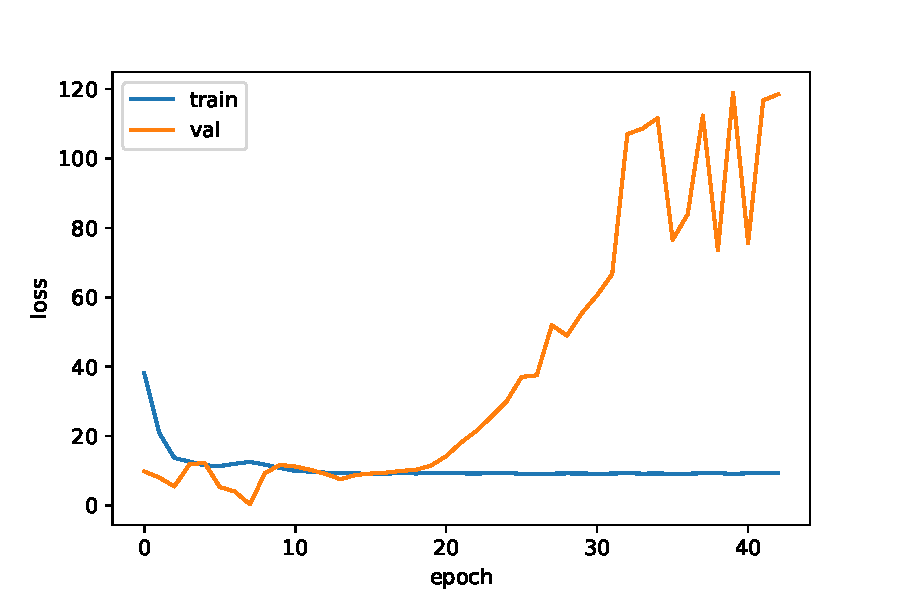
\includegraphics[scale=0.8]{train_val_loss.pdf}}
	\caption{График тренировки 1}
	\label{fig:train1}
\end{figure}
\begin{figure}[h]
	\center{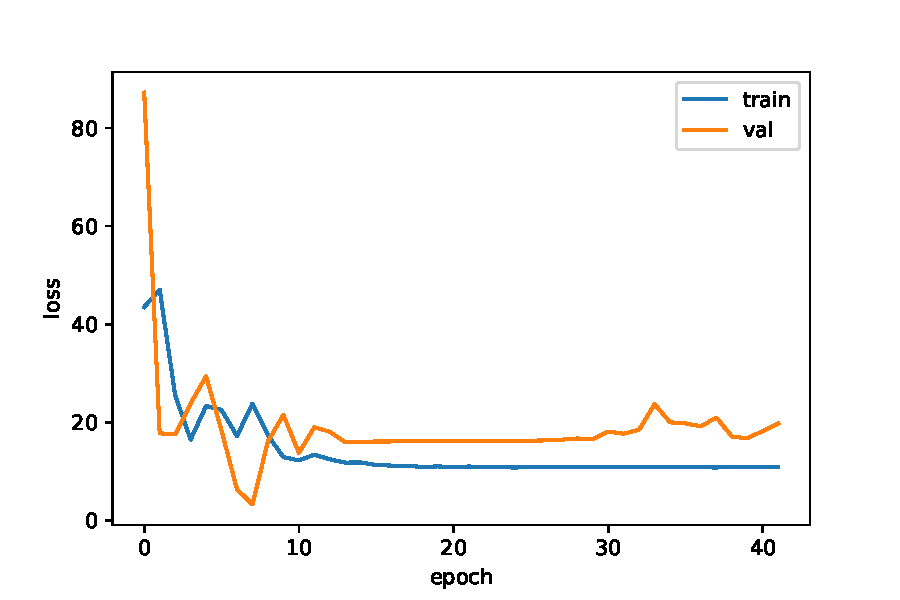
\includegraphics[scale=0.8]{train_val_loss_2.pdf}}
	\caption{График тренировки 2}
	\label{fig:train2}
\end{figure}
Получены они на разных гиперпараметрах. В общем, надо поймать момент, когда лосс на валидации ещё не улетел в небеса. В зависимости от гиперпараметров, он может как на рис.\ref{fig:train2} выйти на плато, а может неконтролируемо расти как на рис.\ref{fig:train1}. Последняя ситуация представляет собой явный overfitting.

В лучшую итерацию лосс на валидации был в районе 0.5, что весьма неплохо, на мой взгляд. Но я потерял эту точку пока экспериментировал, а дедлайн уже поджимает поэтому поставил в качестве критерия лосс на трэйне и валидации меньше 10. Но мне на самом деле повезло!
\begin{figure}[h!]
	\center{
\includegraphics[scale=0.8]{jump.jpg}}
	\caption{Скорее к выводам}
	\label{fig:jump}
\end{figure}

\section*{Итоги}
\addcontentsline{toc}{section}{Итоги}
О везении: нейросеть вышла из цикла тренировки с $MAE = 3.38$ на валидации, что отражено в ноутбуке. Осталось только скормить нейросети все сабмит иксы, вывести всё, в csv и рассчитать MAE. Итоговый $MAE_{final} = 3.39$. Причём, если заглянуть в вывод в Y sub pred.csv Можно заметить, что модель выводит разные числа для разных входных данных, что неплохо.

Да, можно было бы поискать ту самую точку, когда лосс был 0.5. Натыкался на неё несколько раз при разных параметрах. Один раз лосс был даже меньше этого и составлял чуть ли не сотые или тысячные доли, но это было совсем прям один раз. Пруфов, к сожалению, не будет.

Таким образом, написали модельку, способную работать в онлайне, для расчётов ей не нужно несколько часов. Предикт для одного образца — дело нескольких секунд.

Можно ли сделать лосс ещё меньше? Да, безусловно можно. Просто эту конфигурацию нужно поискать.

Можно ли уменьшить склонность к оверфиту? Да, если подключить все нормализации батчей. Но тогда не факт, что мы найдём искомую точку с лоссом меньше единицы.

Как уже было сказано, можно добавить учёт сезонности данных. Это потенциально может дать лучшие результаты.

\section*{Благодарности}
Хочется сказать отдельное спасибо за такое тестовое задание. Без шуток, оно мне показалось крайне занимательным. Получил очень ценный опыт работы с Pytorch на практике. Особенно импонирует тот факт, что за всем этим огромным датасетом стоит реальный производственный физический процесс. Надеюсь этот отчёт был не слишком большой, так что отдельное спасибо, если дочитали до этого момента:)
\end{document}